\documentclass{article}

\textwidth=6.5in
\textheight=8.5in
\voffset=-54pt
\oddsidemargin=0in
\evensidemargin=0in
\setlength{\parskip}{8pt}
\setlength{\parindent}{0pt}

\usepackage{amsmath, amssymb}
\usepackage{ifthen}

\usepackage[inline]{enumitem}
\setlist{topsep=0pt, parsep=8pt}

\usepackage[rgb,table]{xcolor}\convertcolorsUfalse
\usepackage{graphicx}

% change hyperref options
\PassOptionsToPackage{hyphens}{url}
\usepackage[bookmarks,colorlinks,linkcolor=black,citecolor=blue,pdfstartview=FitH,urlcolor=blue]{hyperref}
\hypersetup{pdfpagemode=UseNone}
\usepackage{bookmark}

\usepackage{graphicx}
\usepackage{multicol}
\usepackage{framed}
\usepackage{array}

\usepackage{icomma}

\usepackage{soul}

\usepackage{pgfplots}
\pgfplotsset{compat=1.18}  
\pgfplotscreateplotcyclelist{mycolor}{black, blue, red, green!70!black, magenta, purple, cyan, orange }  
\pgfplotsset{
  disabledatascaling,
  cycle list=tikzcolor, 
  axis lines=middle,
  every axis plot/.style={no marks, thick},
  every axis/.style={
    enlarge x limits=false,
    enlarge y limits=auto,
    xlabel style={at={(current axis.right of origin)},anchor=west},
    ylabel style={at={(current axis.above origin)},anchor=south},
    % extra x and y ticks for asymptotes
    extra x tick style={grid=major, grid style={dashed,black}},
    extra y tick style={grid=major, grid style={dashed,black}},
    /pgf/number format/1000 sep={},
  },    
  tick label style = {font=\footnotesize, fill=\currentbgcolor, inner sep=0pt},    
  xticklabel shift=1pt,    
  scaled ticks=false,
  scaled y ticks=false,
  unbounded coords=jump,
  samples=101,
  minor tick length=0,
  scatter/classes={
    open={mark=*,draw=black,fill=white, mark size=2, thin},
    closed={mark=*,draw=black,fill=black, mark size=2, thin}
  },
  width=3in,
}
\pgfplotsset{open/.style={only marks, mark=*, fill=white, thin, mark size=2}}
\pgfplotsset{closed/.style={only marks, mark=*, draw=black, fill=black,
    thin, mark size=2}}
\pgfplotsset{labeled/.style={nodes near coords, only marks, mark=*, draw=black, fill=black, thin, mark size=2, point meta=explicit symbolic}}

\usepackage{tikz}
\usetikzlibrary{
  matrix,%
  % enables the snake paths
  decorations.pathmorphing,%
  % enables bigger arrows
  decorations.markings,%
  decorations.pathreplacing,%
  decorations.text,%
  calc,%
  patterns,%
  shapes.geometric,%
  arrows,
  decorations.shapes,
  positioning,
  plotmarks,
  intersections
}
\tikzset{>=latex} % sets default arrow type in tikz
\tikzset{font=\normalsize}
\tikzset{mark size=1.5pt, mark options=thin}
\tikzset{pin distance=4pt,
  every pin edge/.style={<-, thin, shorten <= -2pt}}

\interfootnotelinepenalty=10000
\renewcommand{\thefootnote}{(\arabic{footnote})}

\usepackage{multirow, bigdelim}

% change to \usepackage[sols]{handout} to see solutions
\usepackage[sols, notes]{handout}

\newcommand\iscurrentenumi[1]{%
  \ifthenelse{\equal{#1}{\theenumi}}{}{#1}}
\setenumerate[1]{ref=\#\arabic*}
\setenumerate[2]{ref=\protect\iscurrentenumi{\theenumi}(\alph*)}
\newcommand\enumiiprefix[2]{%
  \ifthenelse{{\equal{#1}{\theenumi}}\AND{\equal{#2}{(\alph{enumii})}}}{}{}%
  \ifthenelse{{\equal{#1}{\theenumi}}\AND{\NOT{\equal{#2}{(\alph{enumii})}}}}{#2}{}%
  \ifthenelse{\equal{#1}{\theenumi}}{}{#1#2}%
}
\setenumerate[3]{ref=\protect\enumiiprefix{\theenumi}{(\alph{enumii})}\roman*}

\newlength{\tipmargin}
\makeatletter

\renewenvironment{framed}{
  \setlength{\tipmargin}{\textwidth-\linewidth}
  \advance\@totalleftmargin-\tipmargin
  \def\FrameCommand{\hspace{\tipmargin}\fbox}%
  \advance\linewidth\tipmargin
  \MakeFramed {\advance\hsize-\width \FrameRestore}%
}
{\endMakeFramed}

\makeatother

\definecolor{purple}{rgb}{0.5,0,1.0}

\usepackage{fancyhdr}
\lhead{\textcolor{white}{This content is protected and may not be shared, uploaded, or distributed.}}
\rhead{}
\rfoot{\vspace*{\fill}\footnotesize\textcopyright{} \emph{Harvard Math Ma}}
\renewcommand{\headrulewidth}{0pt}
\pagestyle{fancy}
\begin{document}

\htitle{Continuity}

\begin{problemonly}
  \begin{framed}

You should be able to:
    \begin{itemize}[topsep=0pt,partopsep=0pt,parsep=8pt,itemsep=0pt]
    \item Explain the idea of continuity, both intuitively and precisely using the limit definition.

    \item Use limits to classify discontinuities as \emph{removable discontinuities}, \emph{jump discontinuities}, or \emph{vertical asymptotes}, and describe what each type of discontinuity looks like graphically.

    \item Explain what relationships there are between whether a function is continuous at $a$ and whether it's differentiable at $a$.

    \item Take discontinuities into account when constructing a sign chart for a function. 
    \end{itemize}
  \end{framed}
\end{problemonly}

\begin{enumerate}
\item 

  \note{Students have basically done this already in \href{https://canvas.harvard.edu/courses/138327/files/20852351?wrap=1}{Problem Set 14}, {{\#5}}, although that was worded differently. When we discuss this, the first thing I want students to recognize is that the difference between the functions in (a) and (b) is whether they're continuous at $a$. Then, we'll dive into types of discontinuities.}

  \begin{enumerate}
  \item

    \note{I'm hoping to get examples of different types of discontinuities (removable, jump, vertical asymptote), so when I talk with groups, I will try to ask questions that encourage them to draw ones we're missing.}

    \begin{problem}[\vfill]
      Using white chalk, sketch some functions $f(x)$ for which $\displaystyle \lim_{x \to 3} f(x) \neq f(3)$. Try to draw a few examples that look really different!
    \end{problem}

    \begin{solution} 
      Here are a few examples:
      \begin{center}
        \begin{tikzpicture}
          \begin{axis}[xtick={3}, ytick=\empty, width=2in]
            \addplot+[domain=0:4] {-2*(x-1)*(x-2)*(x-4)+3};
            \addplot+[open] coordinates { (3, 7) };
            \addplot+[closed] coordinates { (3, 3) };
          \end{axis}
        \end{tikzpicture}
        \hspace{0.5in}
        \begin{tikzpicture}
          \begin{axis}[xtick={3}, ytick=\empty, width=2in]
            \addplot+[domain=0:3] {sqrt(x+1)};
            \addplot+[domain=3:4] {-2*(x-1)*(x-2)*(x-4)+3};
            \addplot+[open] coordinates { (3, 7) };
            \addplot+[closed] coordinates { (3, 2) };
          \end{axis}
        \end{tikzpicture}
        \hspace{0.5in}
        \begin{tikzpicture}
          \begin{axis}[xtick=\empty, ytick=\empty, width=2in, extra x
            ticks={3}, ymin=-9, ymax=9] 
            \addplot+[domain=0:4] {-2/(x-3)};
          \end{axis}
        \end{tikzpicture}
      \end{center}
      The first example shows a removable discontinuity at $x = 3$, the
      second shows a jump, and the third shows a vertical asymptote.
    \end{solution}

  \item

    \note{I hope students will come up with an example that isn't differentiable at $x = 3$, but if they don't, that's okay, as we'll see one in \ref{continuous-differentiable-1}.}

    \begin{problem}[\vfill\newpage]
      Using colored chalk, sketch some functions $f(x)$ for which $\displaystyle \lim_{x \to 3} f(x) = f(3)$. Try to draw a few examples that look really different!
    \end{problem}

    \begin{solution} 
      Here are two examples:
      \begin{center}
        \begin{tikzpicture}
          \begin{axis}[xtick={3}, ytick=\empty, width=2in]
            \addplot+[domain=0:2] {sin(deg(x^2/1.05))};
            \addplot+[domain=2:4, samples=201] {sin(deg(x^2/1.05))};
          \end{axis}
        \end{tikzpicture}
        \hspace{0.5in}
        \begin{tikzpicture}
          \begin{axis}[xtick={3}, ytick=\empty, width=2in]
            \addplot+[sharp plot] coordinates { (0, 3) (1, 6) (2, 4) (3,
              7) (4, 5) }; 
          \end{axis}
        \end{tikzpicture}
      \end{center}      
    \end{solution}

  \end{enumerate}

\end{enumerate}
\begin{framed}
  \emph{Limit definitions of continuity / discontinuities}.
  \begin{enumerate}
  \item A function $f(x)$ is continuous at $x = a$ if 
  \fitb{3in}{$\lim\limits_{x \to a} f(x)$ exists and is equal to $f(a)$}.
  \item What are the 3 types of discontinuities we named, and how do we describe each in terms of limits?
    \begin{itemize}[topsep=0pt]
    \item \medskip \solonly{A removable discontinuity aka hole occurs when 
    $\lim\limits_{x \to a} f(x)$ exists but is not equal to $f(a)$.}
    \item \medskip \solonly{A jump discontinuity occurs when 
    $\lim\limits_{x \to a} f(x)$ does not exist, but both one-sided limits exist.}
    \item \medskip \solonly{An infinite discontinuity aka vertical asymptote occurs when 
    at least one one-sided limit is $\pm\infty$.}
    \end{itemize}    
  \end{enumerate}

  \emph{A useful fact.} Any function we can write down with a single (non-piecewise) algebraic formula is continuous at every point in its domain. In other words, the discontinuities of such a function are where it's undefined.
\end{framed}

\begin{enumerate}[resume]
\item 
  \begin{problem}[\vfill]
    Let $f(x) = \dfrac{x - 3}{x - 2}$. Find all values of $x$ in $(-\infty, \infty)$ at which $f$ is discontinuous, and use limits to classify each (that is, to decide whether it's removable, a jump, or a vertical asymptote). 
  \end{problem}

  \begin{solution}
    This function is defined as a single algebraic formula, and so it is continuous
    at every point in its domain. The only value not in its domain is $x=2$. Let's
    consider $\lim\limits_{x \to 2} f(x)$. Direct substitution gives us $\frac{-1}{0}$, 
    which means we are likely dealing with a vertical asymptote. To figure out more, let's
    look at the one-sided limits.

    As $x$ approaches $2$ from the left, the numerator is negative and the denominator is
    negative, so $\lim\limits_{x \to 2^-} \frac{x-3}{x-2} = \infty.$ As $x$ approaches $2$
    from the right, the numerator is negative and the denominator is
    positive, so $\lim\limits_{x \to 2^+} \frac{x-3}{x-2} = -\infty.$ This confirms
    that $x=2$ is a vertical asymptote.
  \end{solution}

\item  \label{continuous-differentiable-1}

  \note{This is practice classifying discontinuities and an opportunity to address confusions about discontinuities vs.\ non-differentiable points.}

  Here's the graph of a function $f(x)$.

  \begin{minipage}[t]{2.1in}
    \vspace{-6pt}
    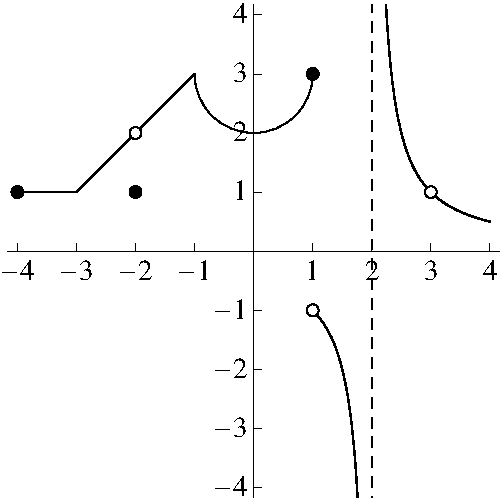
\includegraphics[width=2in]{images/continuous-differentiable-1}
  \end{minipage}
  \begin{minipage}[t]{\linewidth-2.2in}
    \vspace{-12pt}
    \begin{enumerate}
    \item

      \begin{problem}[1in]
        At what values of $x$ in $(-4, 4)$ is $f(x)$ \textit{not} continuous? In other words, at what values of $x$ does $f(x)$ have a discontinuity? What type is each discontinuity?
      \end{problem}

      \begin{solution}
        It has a removable discontinuity at $x = -2$, a jump discontinuity at $x = 1$, a vertical asymptote at $x = 2$, and another removable discontinuity at $x = 3$.
      \end{solution}

    \item

      \note{Sometimes students think functions should be differentiable at removable discontinuities because it feels reasonable to have tangent lines there. If this happens, I will go back to the limit definition of the derivative. For example, $f'(3) = \displaystyle \lim_{h \to 0} \frac{f(3 + h) - f(3)}{h}$ is undefined because $f(3)$ is undefined.}

      \begin{problem}[0.75in]
        At what values of $x$ in $(-4, 4)$ is $f(x)$ \textit{not} differentiable?
      \end{problem}

      \begin{solution}
        It is not differentiable at $x = -3$, $x = -2$, $x = -1$, $x = 1$, $x = 2$, and $x = 3$.
      \end{solution}

    \end{enumerate}    
  \end{minipage}

  \pspace{\newpage}

\item  \label{continuity-differentiability-relationship}

  Decide whether each of the following statements is true or false. If it's false, give an example that shows that it's false (such an example is known as a \textit{counterexample}). 
  \begin{enumerate}
  \item
    \begin{problem}[1in]
      If $f(x)$ is continuous at $x = a$, then $f(x)$ is differentiable at $x = a$.
    \end{problem}

    \begin{solution}
      False; for example, in \ref{continuous-differentiable-1}, $f(x)$ is continuous at $x = -3$, but it is not differentiable at $x = -3$. Any place where $f(x)$ has a ``corner'' is a counterexample.
    \end{solution}

  \item

    \note{If students want some explanation of why this is true, I will give them some intuition: if $f(x)$ is differentiable at $x = a$, then we've seen that, as we zoom in on the graph of $f$ around $x = a$, it looks more and more like the tangent line. And of course, the tangent line is continuous.}

    \begin{problem}[1in]
      If $f(x)$ is differentiable at $x = a$, then $f(x)$ is continuous
      at $x = a$.
    \end{problem}

    \begin{solution}
      This is true.
    \end{solution}

  \end{enumerate}

\item 
  \begin{enumerate}
  \item

    \note{This is basically the idea of the Intermediate Value Theorem, but there's no need to mention the IVT.}

    \begin{problem}[\vfill]
      Can you sketch a function $g(x)$ defined on $[-4, 3]$ which satisfies all 4 of the following properties, or is it impossible?
      \begin{itemize}[nosep]
      \item $g(-4) = 2$
      \item $g(3) = -1$
      \item $g$ has no zeros in $[-4, 3]$
      \item $g$ is continuous on $[-4, 3]$
      \end{itemize}
    \end{problem}

    \begin{solution}
      This is impossible. 
    \end{solution}

  \item
    \begin{problem}[\vfill\newpage]
      Can you sketch a function $g(x)$ defined on $[-4, 3]$ which satisfies the first 3 properties in (a), or is it impossible?
    \end{problem}

    \begin{solution}
      If we get rid of the requirement that the function is continuous, then it's possible:
      \begin{center}
        \begin{tikzpicture}
          \begin{axis}[xtick={-4, 3}, ytick={2, -1}]
            \addplot+[domain=1:3] {-.3*(x-3) -1}; \addplot+[domain=-4:1] {sin(deg(3.14*x))+2}; \addplot[open] coordinates{(1,2)}; \addplot[closed] coordinates{(1,-.4)};
          \end{axis}
        \end{tikzpicture}
      \end{center}
    \end{solution}

  \end{enumerate}

\item  \emph{Summarize.}

  \begin{enumerate}
  \item
    \note{There are two possibilities: $g(a) = 0$ or $g$ has a discontinuity at $a$.}

    \begin{problem}[0.5in]
      If a function $g$ switches from positive to negative or vice versa at $x = a$, what can you say about the behavior of $g$ at $x = a$?
    \end{problem}

    \begin{solution}
      There are two possibilities: $g(a) = 0$, or $g$ has a discontinuity at $a$.
    \end{solution}

\begin{framed}
    This is a specific application of a broader theorem, known as the {\bf Intermediate Value Theorem}, which states that if some function $f$ is continuous on the closed and bounded interval $[a, b]$ and $f(a) = A$ and $f(b)=B$, then somewhere on the interval, $f$ attains every value between $A$ and $B$. (Gottlieb, p.271)
\end{framed}
  \item

    \note{So, when we want to make a sign chart for a function, we really need to look for places where the function is 0 or where it has a discontinuity (which, for functions with a non-piecewise algebraic formula, just means it's undefined).

      This is the last part that's important to cover today.
    }

    \begin{problem}[0.15in]
      If you want to make a sign chart for $g(x)$ and $g(x)$ is given by a single (non-piecewise) algebraic formula, you should start by finding values of $x$ where $g(x)$ is \fitb[$\vphantom{\displaystyle \dfrac{1}{1}}$]{2.5in}{0 or undefined}. 
    \end{problem}

  \end{enumerate}

\item 

  \begin{problem}[\vfill]
    Suppose $f$ is a function with domain $(-\infty, \infty)$, and $f'(x) = \dfrac{x + 2}{\sqrt[3]{x}}$. Where is $f$ decreasing?
  \end{problem}

  \begin{solution}
    Let's make a sign chart for $f'$. We can see that $f'$ is undefined when $x=0$, and
    $f'(x)=0$ when $x=-2$. These values go on our sign chart.

      \begin{center}
        \begin{tikzpicture}
          \draw[<->] (-4, 0) -- (2, 0);
          \node at (-4.5, 0) {$f'(x)$};
          \foreach \x in {-2,0}
            \draw[shift={(\x,0)},color=black] (0pt,3pt) -- (0pt,-3pt) node[below] {$\x$};
          \node[circle, fill=black, inner sep=2pt] at (-2,0) {};
          \node[circle, fill=white, draw=black, inner sep=2pt] at (0,0) {};
        \end{tikzpicture}
      \end{center}

      To determine the sign of $f'(x)$ on each interval, we can test at one $x$-value in
      each interval.
      \begin{alignat*}{3}
      f'(-3) &= \dfrac{-3+2}{\sqrt[3]{-3}} &=\frac{\text{negative}}{\text{negative}} 
      &= \text{positive} \\
      f'(-1) &= \dfrac{-1+2}{\sqrt[3]{-1}} &=\frac{\text{positive}}{\text{negative}}
      &= \text{negative} \\
      f'(1) &= \dfrac{1+2}{\sqrt[3]{1}} &=\frac{\text{positive}}{\text{negative}}
      &= \text{positive}
      \end{alignat*}

      This gives us the following sign chart.
      \begin{center}
        \begin{tikzpicture}
          \draw[<->] (-4, 0) -- (2, 0);
          \node at (-4.5, 0) {$f'(x)$};
          \foreach \x in {-2,0}
            \draw[shift={(\x,0)},color=black] (0pt,3pt) -- (0pt,-3pt) node[below] {$\x$};
          \node[circle, fill=black, inner sep=2pt] at (-2,0) {};
          \node[circle, fill=white, draw=black, inner sep=2pt] at (0,0) {};
          \node[above] at (-3,0) {$+$};
          \node[above] at (-1,0) {$-$};
          \node[above] at (1,0) {$+$};
        \end{tikzpicture}
      \end{center}
      Since $f'$ is negative on the interval $(-2, 0)$, $f$ is decreasing on the interval
      $(-2, 0)$.
  \end{solution}

\item 

  \begin{problem}[\vfill\newpage]
    Let $f(x) = \dfrac{x^2 + 2x}{|x|}$. Find all values of $x$ at which $f(x)$ is discontinuous. For each such value $a$, calculate $\displaystyle \lim_{x \to a^+} f(x)$ and $\displaystyle \lim_{x \to a^-} f(x)$, and use this to classify the discontinuity $a$. 
  \end{problem}

  \begin{solution}
    Since $f(x)$ is an algebraic formula, $f$ is only discontinuous when $f(x)$ is undefined.
    The only value where this occurs is $x=0$. Let's find the one-sided limits as $x \to 0$.

    As $x$ approaches $0$ from the left, since $x$ is negative, $|x| = -x$, so
    \begin{align*}
        \lim_{x\to 0^-} \frac{x^2+2x}{|x|} &= \lim_{x\to 0^-} \frac{x^2+2x}{-x} \\
        &= \lim_{x\to 0^-} -(x+2) \\
        &= -2.
    \end{align*}
    
    As $x$ approaches $0$ from the right, since $x$ is positive, $|x| = x$, so
    \begin{align*}
        \lim_{x\to 0^+} \frac{x^2+2x}{|x|} &= \lim_{x\to 0^+} \frac{x^2+2x}{x} \\
        &= \lim_{x\to 0^+} (x+2) \\
        &= 2.
    \end{align*}

    Since both one-sided limits exist but $\lim\limits_{x \to 0} f(x)$ does not exist,
    $x=0$ is a jump discontinuity.
    
  \end{solution}

\item 
  \begin{problem}[\vfill]
    Let $f(x) =
    \begin{cases}
      x^{2/3} & \text{ if } x < 8 \\
      x - 4 & \text{ if } 8 \leq x \leq 16 \\
      \dfrac{1}{x - 20} & \text{ if } x > 16
    \end{cases}$

    Since $f$ isn't defined by a single formula, what points should we consider if we want to find the discontinuities of $f$? For each such value $a$, use limits to determine whether $f$ is continuous at $a$. If $f$ is not continuous at $a$, determine which type of discontinuity $f$ has there.
  \end{problem}

  \begin{solution}
    Since $f$ isn't defined by a single formula, in addition to any values for which $f(x)$ 
    is undefined, we should consider the endpoints of the various pieces. Thus, we
    should consider the $x$-values $8$, $16$, and $20$. 

    \begin{itemize}

    \item
    First, let's look at $x=8$. As $x$ approaches $8$ from the left, we have
    $\lim\limits_{x \to 8^-} f(x) = \lim\limits_{x \to 8^-} x^{2/3} = 4$. 
    As $x$ approaches $8$ from the right,
    we have $\lim\limits_{x \to 8^+} f(x) =\lim\limits_{x \to 8^+} (x-4) = 4$.
    Since the one-sided limits are equal, the two-sided limit is 
    $\lim\limits_{x \to 8} f(x) =4$. Also, $f(8) = 4$. Since 
    $\lim\limits_{x \to 8} f(x)$ exists and is equal to $f(8)$, $f$ is continuous
    at $x=8$. 
    
    \item
    Now let's look at $x=16$. As $x$ approaches $16$ from the left, we have
    $\lim\limits_{x \to 16^-} f(x) = \lim\limits_{x \to 16^-} (x-4) = 12$. 
    As $x$ approaches $16$ from the right,
    we have $\lim\limits_{x \to 16^+} f(x) =\lim\limits_{x \to 16^+} \frac{1}{x-20}=
    -\frac{1}{4}$. The one-sided limits exist but are not equal, so $f$ has a jump
    discontinuity at $x=16$.

    \item
    Lastly, let's look at $x=20$. As $x$ approaches $20$ from the left, we have
    $\lim\limits_{x \to 20^-} f(x) = \lim\limits_{x \to 20^-} \frac{1}{x-20} = -\infty$. 
    As $x$ approaches $20$ from the right,
    we have $\lim\limits_{x \to 20^+} f(x) =\lim\limits_{x \to 20^+} \frac{1}{x-20}=
    \infty$. Since at least one of the one-sided limits is $\pm \infty$, $f$ has an infinite
    discontinuity at $x=20$, aka a vertical asymptote. 

    \end{itemize}
    
  \end{solution}

\end{enumerate}
\end{document}
